\documentclass[runningheads]{llncs}
\usepackage{graphicx}

\begin{document}
\title{Explain urban regional function}
\author{Submission}

\maketitle 

\begin{abstract}
The abstract should briefly summarize the contents of the paper in
15--250 words.

\keywords{Explanation  \and Urban computing \and Sentiment analysis.}
\end{abstract}
%


\section{Introduction}

\subsection{motivation}
Urban computing is defined by Zheng et al. ~\cite{Zheng2014UrbanConcepts} as an concept where many factors ,such as sensors,prople,vehicles and so on, consist of a dynamic urban system.The aims of urban computing include improve the life level of residents,optimizing urban planning, decreasing traffic jams, reducing various pollution and so on.
With the improvement of living life of urban residents,GPS-embedded taxi begin to play an important part of urban computing.And the data of taxi mobility provide us an valuable way to compute urban system.For example,Zheng et al. ~\cite{Zheng2011taxicabs} detect the flaws in the existing urban planning of a city using the GPS trajectories of taxis traveling in the urban areas. Meng et al.\cite{Meng2017Traffic} propose a framework to infer the city-wide traffic volume information with loop detectors and taxi trajectories.Garg et al.\cite{Garg2018Route}minimizing distance through Monte Carlo tree search to decrease the rate of empty carrying and improve taxi drivers’ profits.
As you can see, Urban computing is closely linked with urban life.

Discovering regions of different function is a step towards urban computing.In this direction,Yuan et al.~\cite{Yuan2012FunctionRegion,Yuan2015FunctionRegion,Yuan2018FunctionRegion} do well in discovering regions of different functions %3 references.
%~\cite{Yuan2012FunctionRegion}~\cite{Yuan2015FunctionRegion}:latent activity trajectories~\cite{Yuan2018FunctionRegion}

\subsection{explain power}
%Previous model
The approaches to explanation recommendation system was developing recently.At the early time,the fundamental methods of personal recommendation is recommendation systems with user-based and item-based. Resnick et al.\cite{Resnick1994UserBased} found user-based collaboration filtering recommendation system.The explanation is the similar neighbors whose interests and rates tend to be consistent with target user.Analogously,Sarwar et al. \cite{Sarwar2001ItemBased} proposed the recommendation with item-based could find the suitable items which has similar features with purchased items.

%model complex, deep model
Variants of these basic model constitute the majority of explanation recommendation systems.e.g.,Pazzani et al.\cite{Pazzani2007ContentBased}
As time going


%data heterogenous 
%explainability -> disadvantage 

%Explaining the result is of crucial importance
We can see that early recommendation systems tend to base on intuition and full with common sense,which improve users' satisfaction easily. Now the explanation recommendation systems is developing with more accuracy , which generate more satisfying results.Nevertheless ,the complexity of models is increasing at the meantime,which covers the intuition of whole structure and weakens the persuasiveness of models.So the explanation is playing an important part in recommendation systems.%~\cite{{Zhang2018SIGIR}}
Majority of users trust and choice satisfaction were highly correlated with the reliability of the explanations for recommendations.Herlocker et al.~\cite{Herlocker2000Explanation}  do an investigation which shows that explanation facilities can improve the acceptance of recommendation systems.The following experiments,e.g.,by Ferwerda et al.~\cite{Ferwerda2012ContentCorrelate} has proven the conclusion.We aim to propose models to explain the destination why we recommend it more persuasively


%explain implementation, we need to incorporate activity and online sentiment
Our goal is to proposed a model to predict taxi destination and provide persuasive explanation for it.
%Furthermore, provide xxx explaination, activity , focus on aspects

\begin{figure}
    \centering
    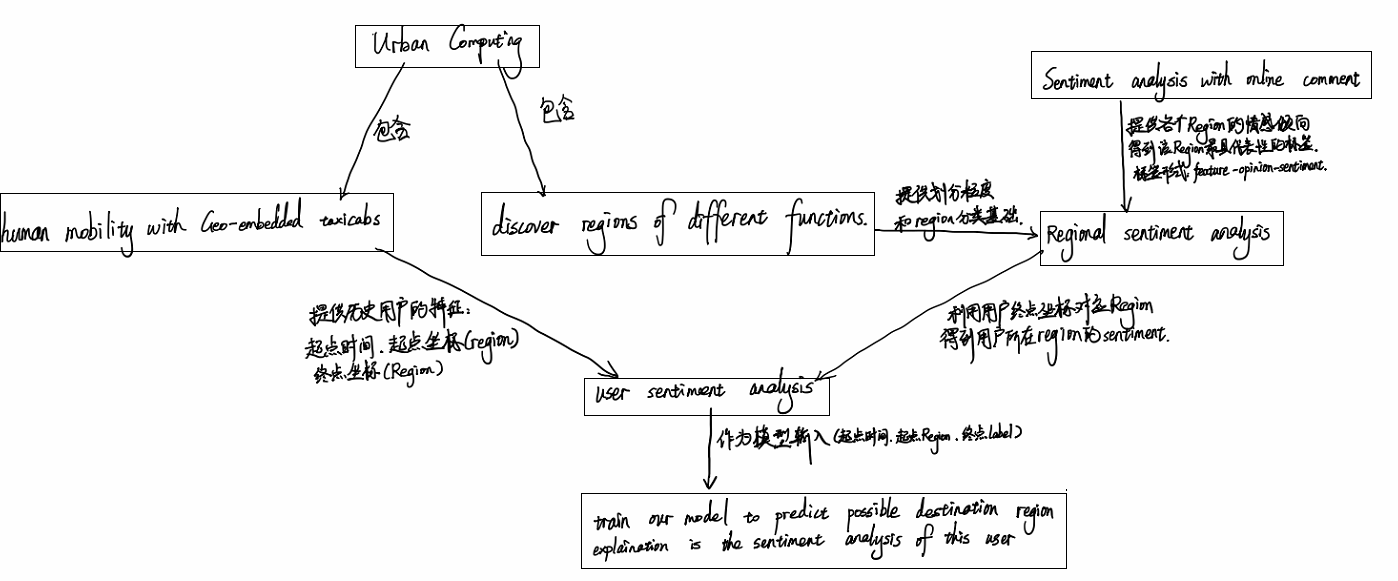
\includegraphics[scale=0.25]{Structure.png}
    \caption{The general structure of our paper}
    %\label{fig:my_label}
\end{figure}

\subsection{problem}
For solve the problem,we face two challenges.One of it is...and the other is ...
segment regions = group regions with similar functions

function = distribution of activitys and opinions

%challenge

previous research



%opinion



%second challenge: time bins



\subsection{contribution}
Our paper has an outstanding result in following several aspect:
\begin{itemize}
  \item According to what I have learned,we are the first one to state-of-the-art
  \item 2
  \item 3
\end{itemize}



\subsection{paper structure}
The remainder of the paper is organized as follows. 
We give an overview for related work in Section 2.
In Section 3, we introduce our novel models as well as proving their logic.
Section 4 presents the suprior result in experiments of our models.
Finally, we made a conclusion and looked forward to our future work in Section 5.

\section{Related Work}

Two lines of work are related to this paper: sentiment analysis into human mobility,content from social media also provide great help for us. Many scholars have made fundamental contributions,and we combined them to find interesting patterns and extended the application .

To the best of our knowledges,we are the first to combined the sentiment into human mobility.

%related work section name, find another suitable name for mobility mining
\subsection{Urban Computing}

Urban computing~\cite{Zheng2014UrbanConcepts} tackles the major issues that cities face by analyzing human mobility collected from different sensors.  
Major sources of human mobility data are checkins in POI~\cite{}, pick-up and drop-off behavior of taxicabs~\cite{} in different locations and  trajectories~\cite{}.
%extract the different among these data
For checkins data, the most commonly adopted model is.
For taxicabs data, to fully utilize pick-up and drop-off, xxx is adopted to enhance xxx
For trajectory data, as it involves multiple points 

%tasks
The aim of mobility mining is to uncover informative patterns of improve incomes of taxi drivers~\cite{}, attracts an increasing research interest~\cite{}. 
However, existing urban computing systems extensively rely on complex machine learning algorithms hence they act as blank-boxes for end users. 
The lack of explainability weakens the persuasiveness and trustworthiness of the system for users
Our work is to provide intuitive explanations of the results for users or system designers
%most of them adopt a topic model, treating mobility patterns as words~\cite{}%topic models



\subsection{Geographical Analysis of Online Sentiment}

Recently, an emrging research interest is witnessed in exploring the geographical factors that affect online sentiment.
Empirical studies have been conducted on large-scale human mobility data, such as checkins~\cite{}, trajectory, xxx~\cite{}
Associations are found between online sentiments and geographical factors, e.g happy regions are more likely to connect with each other~\cite{milan15},a high check-in density region usually presents a more positive moode~\cite{}, 

%complete survey
However, most existing work of this line employ simple statistical analysis to uncover the associations. 
Such a coarse-grained analysis is distorted by latent variables, such as activity of the region.
Our work is the first to incorporate activity to obtain a fine-grained analysis.

\iffalse
\section{Application}
Our models have a wide range of application and their value
\subsection{Billboard}
Billboard
\subsection{Trajectory}
\fi

\section{Experiments}

\subsection{Data Set}
The data set for our experiments including both mobility data and content data.
The mobility data including the pick-up and drop-off time and coordinates in November of the year 2016 provided by DiDi, the biggest taxi platform in China.It contributed to the movement pattern of human mobility.
And the online content is crawled from a website with many comments similar to Yelp called DazhongDianping and a social media named Weibo , which helps sentiment analysis of the regions.

\subsection{Preparation}

\subsection{Baseline and other comparison}

\subsection{Evaluation Metrics}

\subsection{result}

\section{Conclusion}
In this paper , we proposed several models to find the most possible destination region for users and add explanation for it to enhance its persuasiveness.
The models have improve some extra recognition accuracy ,which have an extra contribution for functional city.


\begin{thebibliography}{25}
\bibitem{Zheng2014UrbanConcepts}Zheng Y, Capra L, Wolfson O, et al. Urban Computing:Concepts, Methodologies, and Applications[J]. Acm Transactions on Intelligent Systems \& Technology, 2014, 5(3):1-55.
    %综述城市计算的概念和框架
\bibitem{Zheng2011taxicabs}Zheng Y, Liu Y, Yuan J, et al. Urban computing with taxicabs[C]// International Conference on Ubiquitous Computing. ACM, 2011:89-98.
    %利用GPS轨迹检测出现有城市规划中存在的缺陷。结果包括:1)存在显著交通问题的区域对,2)连接结构以及它们之间的相关性。这些结果可以评估所实施的规划的有效性,例如一个城市新建的公路和地铁线路,并提醒城市规划者在构思未来规划时没有认识到的问题。
\bibitem{Meng2017Traffic} Meng, C.; Yi, X.; Su, L.; Gao, J.; Zheng, Y. City-wide Traffic Volume Inference with Loop Detector Data and Taxi Trajectories. Proceedings of the 25th ACM SIGSPATIAL International Conference on Advances in Geographic Information Systems,ACM,2017, 1:1-1:10 
    %提出了一个框架来推断城市交通流量信息与环路探测器和出租车轨迹。
\bibitem{Garg2018Route}Garg, N.; Ranu, S. Route Recommendations for Idle Taxi Drivers: Find Me the Shortest Route to a Customer! Proceedings of the 24th ACM SIGKDD International Conference on Knowledge Discovery \& 38; Data Mining,ACM,2018, 1425-1434 
    %通过Minimizing Distance through Monte Carlo Tree Search来对出租车司机进行路线推荐,使其提高效率,降低空载率。
\bibitem{Yuan2012FunctionRegion}Yuan J, Zheng Y, Xie X. Discovering regions of different functions in a city using human mobility and POIs[C]// ACM SIGKDD International Conference on Knowledge Discovery and Data Mining. ACM, 2012:186-194.
    %套用LDA,根据功能划分城市区域
\bibitem{Yuan2015FunctionRegion}Yuan N J, Zheng Y, Xie X, et al. Discovering Urban Functional Zones Using Latent Activity Trajectories[J]. Knowledge \& Data Engineering IEEE Transactions on, 2015, 27(3):712-725.
    %
\bibitem{Yuan2018FunctionRegion}Yuan N J, Zheng Y, Xie X. Discovering Functional Zones in a City Using Human Movements and Points of Interest[J]. 2018.
    %
\bibitem{Resnick1994UserBased}Resnick P, Iacovou N, Suchak M, et al. GroupLens:an open architecture for collaborative filtering of netnews[C]// ACM Conference on Computer Supported Cooperative Work. ACM, 1994:175-186.
    %提出user-based collaboration filtering
\bibitem{Sarwar2001ItemBased}Sarwar B, Karypis G, Konstan J, et al. Item-based collaborative filtering recommendation algorithms[C]// International Conference on World Wide Web. ACM, 2001:285-295.
    %提出item-based collaboration filtering
\bibitem{Pazzani2007ContentBased}Pazzani M J, Billsus D. Content-based recommendation systems[M]// The adaptive web. Springer-Verlag, 2007:325-341.
    %提出content-based collaboration filtering    
\bibitem{Alshamsi15milan}Alshamsi A, Awad E, Almehrezi M, et al. Misery loves company: happiness and communication in the city[J]. Epj Data Science, 2015, 4(1):7.
    %把米兰城区划分成100*100区域,根据社交网络发现情绪积极的region更喜欢和其他积极的region交流。
\bibitem{Gallegos16happier}Gallegos L, Huang A, Huang A, et al. Geography of Emotion: Where in a City are People Happier?[C]// International Conference Companion on World Wide Web. International World Wide Web Conferences Steering Committee, 2016:569-574.
    %将其他人的统计方法用于划分区域的签到数据集中,比较得出结论:①签到数据越多的地方积极性越高,消极性越低。②发现在签到数据多的地方签到的用户,活动范围都比较大。可以理解为这个地方比较吸引人,人们愿意走更远的路去这里玩。③结合人口普查的结果,发现签到数据多的地方所居住的居民年龄更大、非西班牙裔人口更多、受教育程度更高
\bibitem{Zhao2016POI}Zhao S, King I, Lyu M R. A Survey of Point-of-interest Recommendation in Location-based Social Networks[J]. 2016.
    %对截止16年最新的50篇与LSBN和POI相关的顶会论文做了一个总结,不知道能不能用上
\bibitem{Zhang2018SIGIR} Zhang, Y.; Zhang, Y.; Zhang, M. SIGIR 2018 Workshop on ExplainAble Recommendation and Search (EARS 2018) //The 41st International ACM SIGIR Conference on Research \& 38; Development in Information Retrieval,ACM,2018, 1411-1413 
    %概述了推荐系统中explanation的重要性
\bibitem{Zhang2018Survey} Zhang Y, Chen X. Explainable Recommendation: A Survey and New Perspectives[J]. 2018.
    %介绍了推荐系统解释的调查概述和未来新视角。主要看了explanation的几种形式
    %基于内容、特征的explanation:利用用户a感兴趣的特征和商品b所拥有的特征来匹配。用户对推荐系统的满意度和信任度与解释高度相关。形式有雷达图等。
    %基于文本的句子形式explanation:在评论等数据中获得更加完善的用户倾向,生成文本句子作为解释。情感抽取工具Sentires(toolkit是一个jre,已得到,未运行),可抽取feature-Opinion-sentiment三元组
\bibitem{Herlocker2000Explanation} Herlocker J L, Konstan J A, Riedl J. Explaining collaborative filtering recommendations[C]// Acm Conference on Computer Supported Cooperative Work. 2000:241-250.
    %为了证明explanation facilities 能提高推荐系统的acceptance,本文通过对210个MovieLens用户的调查,发现绝大部分用户希望在推荐结果中加入explanation。
    %
\bibitem{Ferwerda2012ContentCorrelate} Ferwerda B, Swelsen K, Yang E. Explaining Content-Based Recommendations[J]. Bruceferwerda Com.
    %这篇只发表在作者自己的网站上,但是有被引用。内容是选择过多时,用户满意度会下降。这篇文章通过实验证明,用户的满意度和解释性有关。
    %
\bibitem{Zhang2015Sentires}  Zhang Y, Zhang M, Liu Y, et al. Boost Phrase-level Polarity Labelling with Review-level Sentiment Classification[J]. Computer Science, 2015.
    %开发了一个情感抽取工具Sentires,在短语这个级别层面上做情感极性标注。可以从某个产品领域的产品评论中抽取“feature-oppion-sentiment”这样的三元组。例如,在手机领域,“noise-high-negative”,“screen-clear-positive”等。
    %对于我们的大众点评数据,也可以“feature-opinion-sentiment”。其中feature表示52个标签,opinion表示评分,sentiment表示根据评分是积极or消极(与feature其实无关)
\bibitem{Costa2017LSTM} Costa F, Ouyang S, Dolog P, et al. Automatic Generation of Natural Language Explanations[J]. 2017.
    %提出了一个LSTM模型来生成评论。并提出八个评估生成文字可读性的测量标准
\bibitem{}
    %
    %
\bibitem{}
    %
    %
\bibitem{}
    %
    %
\bibitem{}
    %
    %
\end{thebibliography}
\end{document}
